\documentclass[a4paper, 12pt]{scrartcl}
\usepackage[utf8]{inputenc}
\usepackage[ngerman]{babel}
\usepackage[T1]{fontenc}
\usepackage{graphicx}
\usepackage{hyperref}

\hypersetup{
	colorlinks=true,
	linkcolor=blue,
	filecolor=blue,      
	urlcolor=blue,
	pdftitle={ Example},
	pdfpagemode=FullScreen,
}

\title{End-2-End-Prozess}
\titlehead{Praxisbericht}
\author{Maksym Mykhailych}
\date{09. September 2025}

\begin{document}
	\maketitle
	\newpage 	
	\tableofcontents
	\newpage
	%\section{Abstract}
	
	\newpage
	\section{Einleitung}
	Einleitender Text.
	\newpage
	\subsection{Motivation}
	\subsection{Aufgabenstellung}
	\subsection{Aufbau der Arbeit}
	Text.
	\newpage
	\section{Grundlagen}
	\subsection{Vorstellung von Capgemini}
	\subsubsection{Gesamtheitliche Darstellung von Capgemini} %VOrstellung von Capgemini(Geschichte, Zahlen, Wie groß?)
Capgemini, mit Hauptsitz in Paris, ist ein transnationales, börsennotiertes Unternehmen, das Beratungs-, Technologiedienstleistungen und digitale Transformationslösungen anbietet. Das Unternehmen bietet eine Vielzahl von Dienstleistungen, darunter Beratung, Technologie und Outsourcing. Mit einer Präsenz in über 50 Ländern bedient Capgemini Kunden aus diversen Branchen, einschließlich Finanzdienstleistungen, Automobilindustrie, Gesundheitswesen und Einzelhandel. Im \href{https://www.capgemini.com/de-de/news/pressemitteilung/capgemini-delivers-another-record-performance-in-2023/}{Jahr 2023} erzielte Capgemini einen Umsatz von 22,5 Milliarden Euro und beschäftigt weltweit etwa 340.000 Mitarbeiter, davon rund 12.500 in Deutschland laut der internen Daten.
	\begin{figure}[h!]
		\begin{center}
			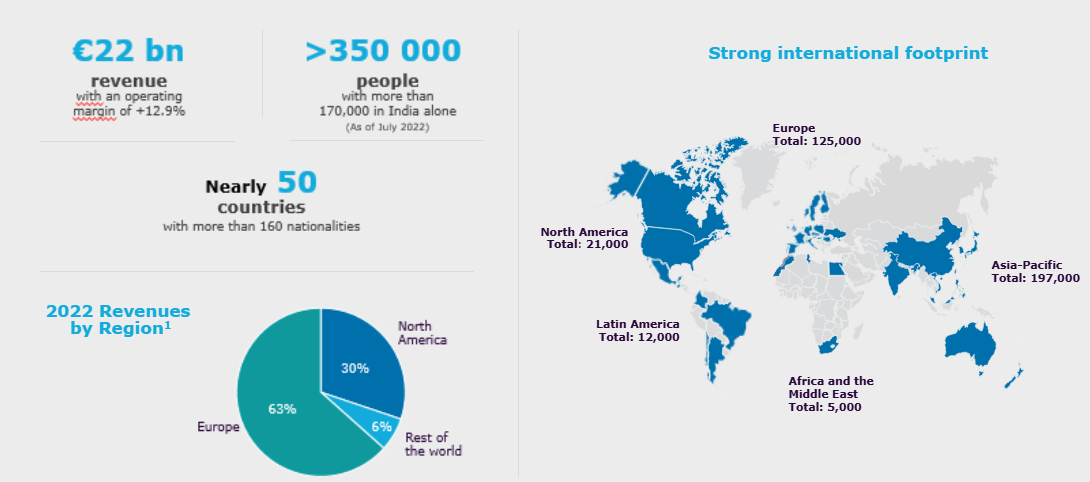
\includegraphics[width=12cm]{CApgemini zahlen.png}
			\caption{Stand von Capgemini zu 2023}
			\label{Stand von Capgemini}
		\end{center}
	\end{figure}
	\subsubsection{Struktur und Organisation in Deutschland}

Capgemini Gruppe bietet ihren Kunden eine End-to-End-IT-Transformation, die von der Umgestaltung komplexer IT-Architekturen bis hin zur Entwicklung spezifischer kleiner Funktionen reicht. In diesem Zusammenhang verfügt Capgemini über große Mitarbeiteranzahl und besteht aus mehreren \href{https://www.capgemini.com/de-de/unternehmen/wer-wir-sind/unsere-marken/}{ Marken}:
	\begin{itemize}
		\item \textbf{Capgemini:} Das Mutterunternehmen bietet ein breites Spektrum an Dienstleistungen, darunter IT-Beratung und Technologie-Services.
		
		\item \textbf{Capgemini Invent:} Diese Sparte konzentriert sich auf die strategische digitale Entwicklung der Kunden.
		\item \textbf{Capgemini Engineering:} Ein weltweit führender Anbieter von Engineering- und F\&E-Dienstleistungen, der Kunden dabei unterstützt, ihren Weg zur Intelligent Industry zu beschleunigen.
		\item \textbf{Sogeti:} Entwickelt, testet und schützt innovative Anwendungen für Unternehmen und stützt sich dabei auf Expertise in den Bereichen Beratung, Testen, agile und Cloud-Entwicklung sowie Cybersicherheit.
	\end{itemize}
Dies sind die wichtigsten Marken von Capgemini in Deutschland. Meine Erfahrung habe ich im Mutterunternehmen von Capgemini gesammelt, wo das Unternehmen auch intern in verschiedene Abteilungen unterteilt ist. Meine Tätigkeit fand in der Abteilung statt, die paketbasierte Lösungen %Im glossar erklären was PBS ist(SAP, Windchill etc.)
  für Kunden anbietet.


	\newpage
	\subsection{Definition des End-2-End-Prozesses}
	\subsubsection{Überblick des allgemeinen End-2-End-Prozesses} %wie sieht algemein E2E-Prozess bei der Beratung!

	\subsubsection{End-2-End-Prozess bei Capgemini}
	\newpage
	\subsection{PLM-Systeme}
	\subsubsection{Allgemeine Übersicht der PLM-Systeme}
	\section*{\normalsize Definition und Bedeutung der Produkt Lebenzyclus Managment(PLM)}
Das Auto ist heutzutage ein unverzichtbarer Begleiter des Menschen, der ihn bei der schnellen Fortbewegung unterstützt. Aus der Sicht eines Ingenieurs jedoch ist es eine komplexe Maschine, die aus Hunderttausenden von Einzelteilen besteht, die effizient verwaltet werden müssen. In diesem Zusammenhang entstand zu Beginn des 21. Jahrhunderts ein neues Paradigma in Fertigungsunternehmen: das Product Lifecycle Management (PLM). PLM ermöglicht es Unternehmen, ihre Produkte während des gesamten Lebenszyklus zu überwachen und zu steuern. Das ist eine der wichtigsten Aktivitäten der Fertigungsunternehmen.
	\begin{figure}[h!]
	\begin{center}
		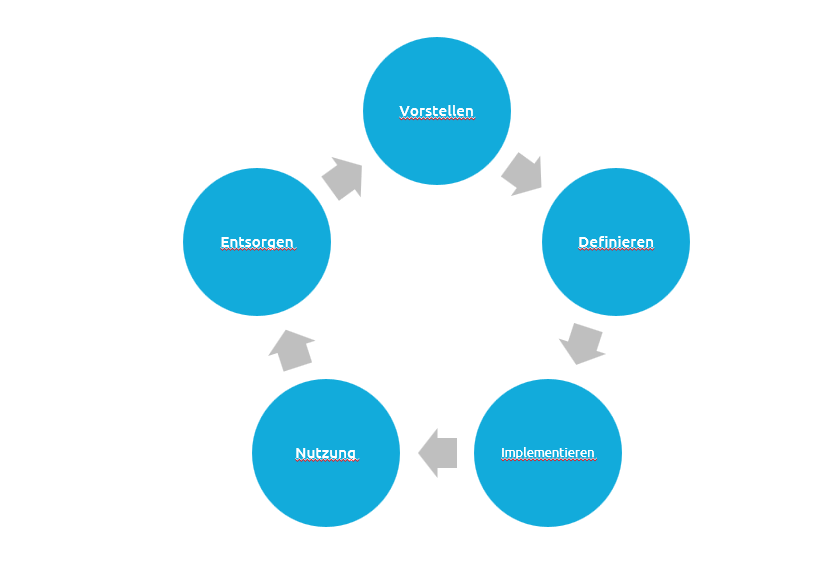
\includegraphics[width=12cm]{PLM.png}
		\caption{Visualisierung von Product Lifecycle Management}
		\label{PLM}
	\end{center}
\end{figure}%Nach fotos fragen!!!
\newline

Wenn ein Unternehmen die Kontrolle über ein Produkt verliert, können schwerwiegende Probleme auftreten, die katastrophale Konsequenzen haben können. Der Verlust der Kontrolle kann zu Produktionsverzögerungen führen, was finanzielle Verluste für das Unternehmen zur Folge hat. Darüber hinaus kann die mangelnde Kontrolle über die Produktion zu Unzufriedenheit bei den Kunden führen oder sogar gesundheitliche Probleme verursachen.\cite{stark2011product}
	\subsubsection{Vorstellung von verschiedenen Vendoren}
	Text.
	\newpage
	\section{Durchführung}
	\subsection{Phase 1: Sales} 
	\subsubsection{Ausgangslage und Aufgabenstallung} %Ich beschäftige mich mit der Showcase für die Kunden um das Projekt zu kriegen.
	\subsubsection{Anforderungen für die Erstellung der Demonstratorenübersicht} %welche versionen die Demonstratoren haben, Ziel des Demonstrators, Beschreibungen etc.
	\subsubsection{Tools-Analyse}%Welche Tools gibt und welche sind geeignet für meinen Demostrator(Beschränung von Unternehmen betrachten)
	\subsubsection{Erstellung der Demonstratorenübersicht}
	\newpage
	\subsection{Phase 2: Staffing}
	\subsubsection{Relevanz der Staffing für Capgemini}%was lebenswichtiges macht Christoph
	\subsubsection{Ausgangslage und Aufgabenstellung}
	\subsubsection{Anforderungen fürs Reporting}
	\subsubsection{Umsetzung des Berichtswesen...}
	\newpage
	\subsection{Phase 3: Projektplanung}
	\newpage
	\subsection{Phase 4: Delivery}
	\newpage
	\subsection{Phase 5: Closure}
	\newpage
	\section{Auswertung}
	\subsection{Validierung der Anforderung}%für PLM
	\newpage
	\section{Ergebnisse und Diskussion}
		\newpage
	\section{Ausblick}
	asdasdasdasda~\cite{karmasin2017gestaltung}
	asdasdasdasda~\cite{example2025}
		\newpage
	\section{Anhang}
	\bibliographystyle{plain}
	\bibliography{Gestaltung_wissenschaftlicher_Arbeit.bib}
	\subsection{Anforderungen für das Showcase}
	\begin{itemize}
		\item Zielsetung und Planung
		\item Infrstraktur aufbauen
		\subitem PDM-systeme und PLM-software auswählen
		\subitem CAD-Tools integrieren
		\subitem ERP-Systeme 
		\item Erstellung der Demonstrationsdaten
		\subitem Beispielprodukt entwickeln nach Zielsetzung
		\subitem Stückliste für das Produkt vorbereiten
		\item Visualisierung entwickeln
		\item Tests durchführen
		\item Präsentation für die Entwicklung des Beispielprodukts vorbereiten 
	\end{itemize}
\end{document}